% Use only LaTeX2e, calling the article.cls class and 12-point type.

\documentclass[12pt]{article}

% Users of the {thebibliography} environment or BibTeX should use the
% scicite.sty package, downloadable from *Science* at
% www.sciencemag.org/about/authors/prep/TeX_help/ .
% This package should properly format in-text
% reference calls and reference-list numbers.

\usepackage{scicite}

% Use times if you have the font installed; otherwise, comment out the
% following line.

\usepackage{times}

% The preamble here sets up a lot of new/revised commands and
% environments.  It's annoying, but please do *not* try to strip these
% out into a separate .sty file (which could lead to the loss of some
% information when we convert the file to other formats).  Instead, keep
% them in the preamble of your main LaTeX source file.

\usepackage{graphicx}

% The following parameters seem to provide a reasonable page setup.

\topmargin 0.0cm
\oddsidemargin 0.2cm
\textwidth 16cm 
\textheight 21cm
\footskip 1.0cm


%The next command sets up an environment for the abstract to your paper.

\newenvironment{sciabstract}{%
\begin{quote} \bf}
{\end{quote}}


% If your reference list includes text notes as well as references,
% include the following line; otherwise, comment it out.

\renewcommand\refname{References and Notes}

% The following lines set up an environment for the last note in the
% reference list, which commonly includes acknowledgments of funding,
% help, etc.  It's intended for users of BibTeX or the {thebibliography}
% environment.  Users who are hand-coding their references at the end
% using a list environment such as {enumerate} can simply add another
% item at the end, and it will be numbered automatically.

\newcounter{lastnote}
\newenvironment{scilastnote}{%
\setcounter{lastnote}{\value{enumiv}}%
\addtocounter{lastnote}{+1}%
\begin{list}%
{\arabic{lastnote}.}
{\setlength{\leftmargin}{.22in}}
{\setlength{\labelsep}{.5em}}}
{\end{list}}


% Include your paper's title here

\title{Interim Report} 


% Place the author information here.  Please hand-code the contact
% information and notecalls; do *not* use \footnote commands.  Let the
% author contact information appear immediately below the author names
% as shown.  We would also prefer that you don't change the type-size
% settings shown here.

\author
{Radek Chramosil\\
\\
\normalsize{WorldQuant University}\\
\\
\normalsize{E-mail:  radek@keemail.me}
}

% Include the date command, but leave its argument blank.

\date{}



%%%%%%%%%%%%%%%%% END OF PREAMBLE %%%%%%%%%%%%%%%%



\begin{document} 

% Double-space the manuscript.

\baselineskip24pt

% Make the title.

\maketitle 



% Place your abstract within the special {sciabstract} environment.

\begin{sciabstract}
This document is the Interim Report for the Capstone Project. It shows the basic structure for the database that holds data the data from crypto-currency exchange Binance and some initial data analysis.
\end{sciabstract}

% In setting up this template for *Science* papers, we've used both
% the \section* command and the \paragraph* command for topical
% divisions.  Which you use will of course depend on the type of paper
% you're writing.  Review Articles tend to have displayed headings, for
% which \section* is more appropriate; Research Articles, when they have
% formal topical divisions at all, tend to signal them with bold text
% that runs into the paragraph, for which \paragraph* is the right
% choice.  Either way, use the asterisk (*) modifier, as shown, to
% suppress numbering.

\section*{Introduction}
The structure of the database is described below. Additionally,  I provide more details about the data analyses so far carried out as well as some suggestion for trading possible trading strategies. Some plots for second data set are provided. The asset I worked with is \textbf{TUSDBTC} as quoted on \textit{Binance Exchange}. The asset is Bitcoin quoted in USD. The access to the full exchange is free and level 2 data is available for every tick.
I was not sure how to set up and event that the code would run each time there is trade on the exchange.

\pagebreak

\section*{Database Structure}
I have included the below tables in this submission. The tables can be created by SQL commands in the ``create\_db.sql`` file. The schema for the database is shows in Figure \ref{fig:schema}.\\
\begin{figure}[h!]
  \centering
  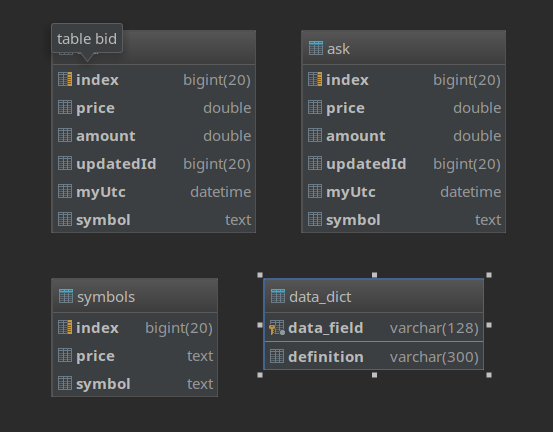
\includegraphics[scale=0.40]{schema.png}
  \caption{Schema}
  \label{fig:schema}
\end{figure}

The tables can be dropped using the ``rollback\_db.sql`` file. This file provides a logical inverse to the create operation. Additionally, I built functionality that can create table on fly using Pandas and SQL Alchemy however the default behaviours are not very good as it fails to create foreign keys and so on.

\subsection*{Tables}
\paragraph*{symbolRef.} This is just a reference table for symbols. The symbols are strings, however it is more efficient to use integers for foreign keys and it is better to store integers than strings.
\paragraph*{bid and ask.} These to table are identical from data types point of view however the just store the bid and ask prices as well as my UTC time stamp and the server `updatedId` flag. This is a large integer that gets changed each time there is a trade.
\paragraph*{limits.}. Basically, the exchange give users request or order limits in time intervals. We can make 1200 data request in a minute or 10 orders in a second and 100 000 orders in a day. If we are creating a real trading application we would have to consider these closely.
\paragraph*{data\_dict.} This is manually created table and holds descriptions for the data fields in the database.

\section*{Bid and Ask}
Bid and ask prices are split into two tables. The tables are identical. The tables from Figure \ref{fig:ask} and Figure \ref{fig:bid} carry the data for the symbol and specific Exchange ID as given by \textit{updateId} column. My time stamps are in the \textit{myUtc} column representing the time on my computer.

\begin{figure}[h!]
	\centering
  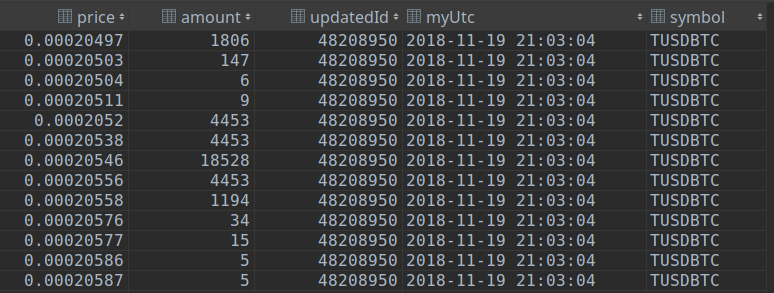
\includegraphics[scale=0.3]{ask.png}
  \caption{Ask Price}
  \label{fig:ask}
\end{figure}

\begin{figure}[h!]
	\centering
  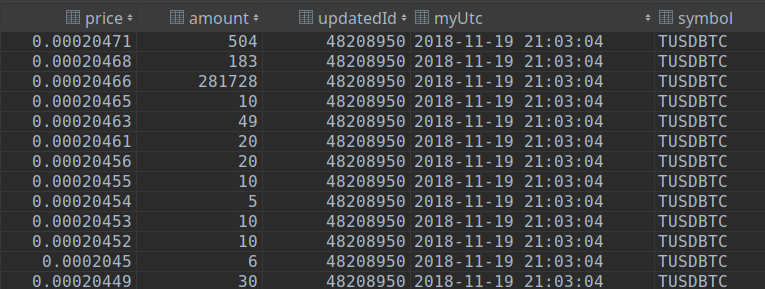
\includegraphics[scale=0.3]{bid.png}
  \caption{Bid Price}
  \label{fig:bid}
\end{figure}

\section*{Exchange API}
It is important to handle the communication to the Exchange well. The class \textit{DataEndPoint} hold all methods that can collect the data from the exchange as opposed to submit trades. I leave it to the reader to read over the comments for these methods to see what can be easily pulled out from the exchange.

\section*{Data Analysis - First Look}
I collected 1 hour of trading data on per second basis. Figure \ref{fig:plt1} shows cumulative bid and ask prices with quantity. The way how I think about this is it is supply and demand curves. We see that there is a lot of volatility over 1 minute interval. This is good as it means that we will be able to create strategies.
\begin{figure}[h!]
	\centering
  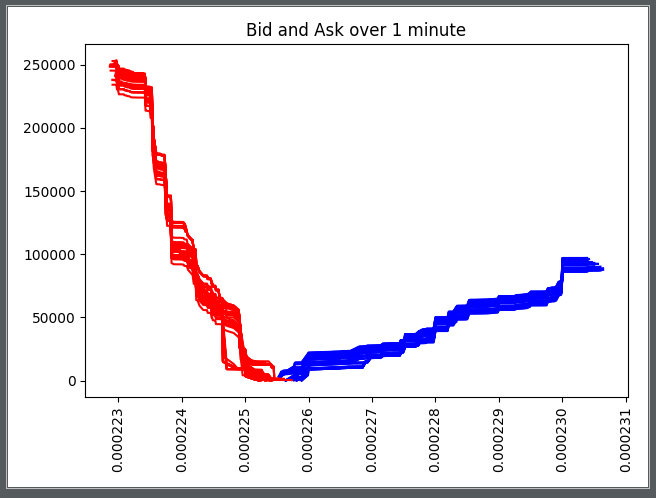
\includegraphics[scale=0.5]{plot1.png}
  \caption{All bid and ask prices and quantities in 1 minute}
  \label{fig:plt1}
\end{figure}

The problem in the Figure \ref{fig:plt1} is that we do not see much details. So, I plotted the same time interval but with close look at what was happing around the spread in Figure \ref{fig:plt2}. Again we see the volatility in the price within one minute.

\begin{figure}[h!]
	\centering
  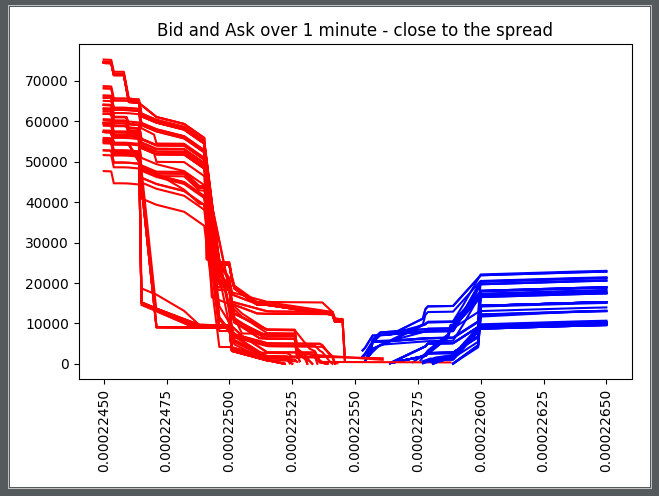
\includegraphics[scale=0.5]{plot2.png}
  \caption{Detailed Price and quantity moments around the spread in 1 minute}
  \label{fig:plt2}
\end{figure}

We also have have look the maximum bid and minimum ask prices and plot them over the 1 hour interval. This is plotted in Figure \ref{fig:plt3}. This shows that we do have trends and turning points happing over time again. We should use the trading strategies that we learning for this and we can starting simulating the trade at bid and ask prices.

\begin{figure}[h!]
	\centering
  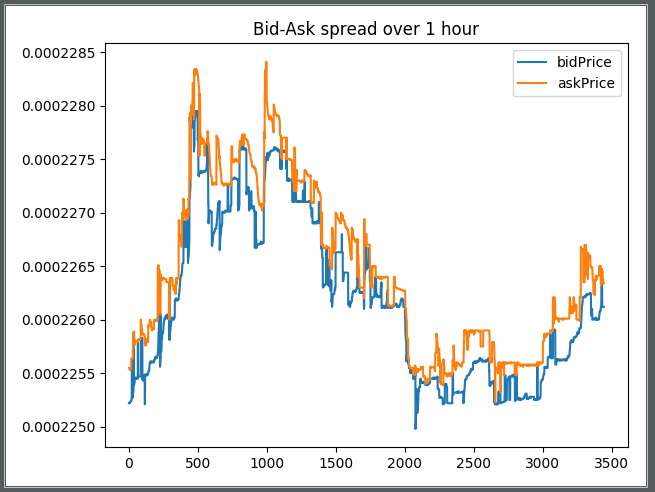
\includegraphics[scale=0.5]{plot3.png}
  \caption{Max bid and min ask over 1 hour}
  \label{fig:plt3}
\end{figure}

Finally, we check the spread for the two currencies as in Figure \ref{fig:plt4}. We immediately see that that we could create mean reversion strategy for the spread. It may not be viable on profit versus fee basis however we could tests this.

\begin{figure}[h!]
	\centering
  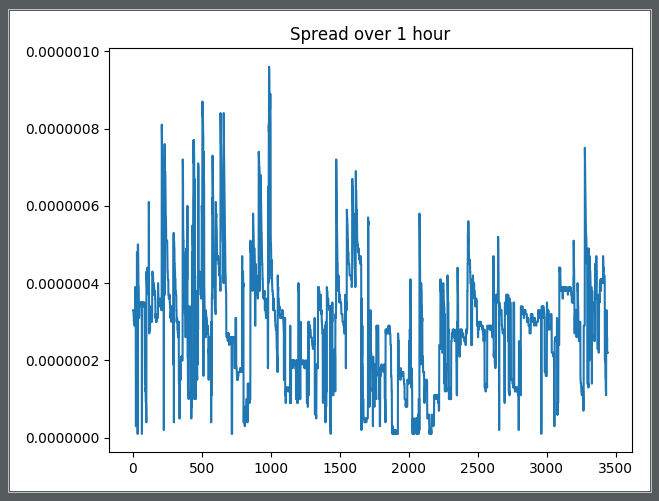
\includegraphics[scale=0.5]{plot4.png}
  \caption{Max bid and min ask spread over 1 hour}
  \label{fig:plt4}
\end{figure}

\pagebreak
\section*{Summary}
Looking at the data, it is easy to spot the same patters as in the time frequencies however connecting to the exchange directly gives full details as to what is going in the market. We are not able to do this for equity or standard financial markets for free. Having a look at the data, we will be able to exactly model what is going in the market rather than second guess from some summary data such as OHLC from Yahoo.

\section*{Formatting Citations}

Citations can be handled in one of three ways.  The most
straightforward (albeit labor-intensive) would be to hardwire your
citations into your \LaTeX\ source, as you would if you were using an
ordinary word processor.  Thus, your code might look something like
this:


\begin{quote}
\begin{verbatim}
However, this record of the solar nebula may have been
partly erased by the complex history of the meteorite
parent bodies, which includes collision-induced shock,
thermal metamorphism, and aqueous alteration
({\it 1, 2, 5--7\/}).
\end{verbatim}
\end{quote}


\noindent Compiled, the last two lines of the code above, of course, would give notecalls in {\it Science\/} style:

\begin{quote}
\ldots thermal metamorphism, and aqueous alteration ({\it 1, 2, 5--7\/}).
\end{quote}

Under the same logic, the author could set up his or her reference list as a simple enumeration,

\begin{quote}
\begin{verbatim}
{\bf References and Notes}

\begin{enumerate}
\item G. Gamow, {\it The Constitution of Atomic Nuclei
and Radioactivity\/} (Oxford Univ. Press, New York, 1931).
\item W. Heisenberg and W. Pauli, {\it Zeitschr.\ f.\ 
Physik\/} {\bf 56}, 1 (1929).
\end{enumerate}
\end{verbatim}
\end{quote}

\noindent yielding

\begin{quote}
{\bf References and Notes}

\begin{enumerate}
\item G. Gamow, {\it The Constitution of Atomic Nuclei and
Radioactivity\/} (Oxford Univ. Press, New York, 1931).
\item W. Heisenberg and W. Pauli, {\it Zeitschr.\ f.\ Physik} {\bf 56},
1 (1929).
\end{enumerate}
\end{quote}

That's not a solution that's likely to appeal to everyone, however ---
especially not to users of B{\small{IB}}\TeX\ \cite{inclme}.  If you
are a B{\small{IB}}\TeX\ user, we suggest that you use the
\texttt{Science.bst} bibliography style file and the
\texttt{scicite.sty} package, both of which we are downloadable from our author help site
(http://www.sciencemag.org/about/authors/prep/TeX\_help/).  You can also
generate your reference lists by using the list environment
\texttt{\{thebibliography\}} at the end of your source document; here
again, you may find the \texttt{scicite.sty} file useful.

Whether you use B{\small{IB}}\TeX\ or \texttt{\{thebibliography\}}, be
very careful about how you set up your in-text reference calls and
notecalls.  In particular, observe the following requirements:

\begin{enumerate}
\item Please follow the style for references outlined at our author
  help site and embodied in recent issues of {\it Science}.  Each
  citation number should refer to a single reference; please do not
  concatenate several references under a single number.
\item Please cite your references and notes in text {\it only\/} using
  the standard \LaTeX\ \verb+\cite+ command, not another command
  driven by outside macros.
\item Please separate multiple citations within a single \verb+\cite+
  command using commas only; there should be {\it no space\/}
  between reference keynames.  That is, if you are citing two
  papers whose bibliography keys are \texttt{keyname1} and
  \texttt{keyname2}, the in-text cite should read
  \verb+\cite{keyname1,keyname2}+, {\it not\/}
  \verb+\cite{keyname1, keyname2}+.
\end{enumerate}

\noindent Failure to follow these guidelines could lead
to the omission of the references in an accepted paper when the source
file is translated to Word via HTML.

\section*{Handling Math, Tables, and Figures}

Following are a few things to keep in mind in coding equations,
tables, and figures for submission to {\it Science}.

\paragraph*{In-line math.}  The utility that we use for converting
from \LaTeX\ to HTML handles in-line math relatively well.  It is best
to avoid using built-up fractions in in-line equations, and going for
the more boring ``slash'' presentation whenever possible --- that is,
for \verb+$a/b$+ (which comes out as $a/b$) rather than
\verb+$\frac{a}{b}$+ (which compiles as $\frac{a}{b}$).  Likewise,
HTML isn't tooled to handle certain overaccented special characters
in-line; for $\hat{\alpha}$ (coded \verb+$\hat{\alpha}$+), for
example, the HTML translation code will return [\^{}$(\alpha)$].
Don't drive yourself crazy --- but if it's possible to avoid such
constructs, please do so.  Please do not code arrays or matrices as
in-line math; display them instead.  And please keep your coding as
\TeX-y as possible --- avoid using specialized math macro packages
like \texttt{amstex.sty}.

\paragraph*{Displayed math.} Our HTML converter sets up \TeX\
displayed equations using nested HTML tables.  That works well for an
HTML presentation, but Word chokes when it comes across a nested
table in an HTML file.  We surmount that problem by simply cutting the
displayed equations out of the HTML before it's imported into Word,
and then replacing them in the Word document using either images or
equations generated by a Word equation editor.  Strictly speaking,
this procedure doesn't bear on how you should prepare your manuscript
--- although, for reasons best consigned to a note \cite{nattex}, we'd
prefer that you use native \TeX\ commands within displayed-math
environments, rather than \LaTeX\ sub-environments.

\paragraph*{Tables.}  The HTML converter that we use seems to handle
reasonably well simple tables generated using the \LaTeX\
\texttt{\{tabular\}} environment.  For very complicated tables, you
may want to consider generating them in a word processing program and
including them as a separate file.

\paragraph*{Figures.}  Figure callouts within the text should not be
in the form of \LaTeX\ references, but should simply be typed in ---
that is, \verb+(Fig. 1)+ rather than \verb+\ref{fig1}+.  For the
figures themselves, treatment can differ depending on whether the
manuscript is an initial submission or a final revision for acceptance
and publication.  For an initial submission and review copy, you can
use the \LaTeX\ \verb+{figure}+ environment and the
\verb+\includegraphics+ command to include your PostScript figures at
the end of the compiled PostScript file.  For the final revision,
however, the \verb+{figure}+ environment should {\it not\/} be used;
instead, the figure captions themselves should be typed in as regular
text at the end of the source file (an example is included here), and
the figures should be uploaded separately according to the Art
Department's instructions.


\section*{What to Send In}

What you should send to {\it Science\/} will depend on the stage your manuscript is in:

\begin{itemize}
\item {\bf Important:} If you're sending in the initial submission of
  your manuscript (that is, the copy for evaluation and peer review),
  please send in {\it only\/} a PostScript or PDF version of the
  compiled file (including figures).  Please do not send in the \TeX\ 
  source, \texttt{.sty}, \texttt{.bbl}, or other associated files with
  your initial submission.  (For more information, please see the
  instructions at our Web submission site,
  http://www.submit2science.org/ .)
\item When the time comes for you to send in your revised final
  manuscript (i.e., after peer review), we require that you include
  all source files and generated files in your upload.  Thus, if the
  name of your main source document is \texttt{ltxfile.tex}, you
  need to include:
\begin{itemize}
\item \texttt{ltxfile.tex}.
\item \texttt{ltxfile.aux}, the auxilliary file generated by the
  compilation.
\item A PostScript file (compiled using \texttt{dvips} or some other
  driver) of the \texttt{.dvi} file generated from
  \texttt{ltxfile.tex}, or a PDF file distilled from that
  PostScript.  You do not need to include the actual \texttt{.dvi}
  file in your upload.
\item From B{\small{IB}}\TeX\ users, your bibliography (\texttt{.bib})
  file, {\it and\/} the generated file \texttt{ltxfile.bbl} created
  when you run B{\small{IB}}\TeX.
\item Any additional \texttt{.sty} and \texttt{.bst} files called by
  the source code (though, for reasons noted earlier, we {\it
    strongly\/} discourage the use of such files beyond those
  mentioned in this document).
\end{itemize}
\end{itemize}

% Your references go at the end of the main text, and before the
% figures.  For this document we've used BibTeX, the .bib file
% scibib.bib, and the .bst file Science.bst.  The package scicite.sty
% was included to format the reference numbers according to *Science*
% style.


\bibliography{scibib}

\bibliographystyle{Science}



% Following is a new environment, {scilastnote}, that's defined in the
% preamble and that allows authors to add a reference at the end of the
% list that's not signaled in the text; such references are used in
% *Science* for acknowledgments of funding, help, etc.

\begin{scilastnote}
\item We've included in the template file \texttt{scifile.tex} a new
environment, \texttt{\{scilastnote\}}, that generates a numbered final
citation without a corresponding signal in the text.  This environment
can be used to generate a final numbered reference containing
acknowledgments, sources of funding, and the like, per {\it Science\/}
style.
\end{scilastnote}




% For your review copy (i.e., the file you initially send in for
% evaluation), you can use the {figure} environment and the
% \includegraphics command to stream your figures into the text, placing
% all figures at the end.  For the final, revised manuscript for
% acceptance and production, however, PostScript or other graphics
% should not be streamed into your compliled file.  Instead, set
% captions as simple paragraphs (with a \noindent tag), setting them
% off from the rest of the text with a \clearpage as shown  below, and
% submit figures as separate files according to the Art Department's
% instructions.


\clearpage

\noindent {\bf Fig. 1.} Please do not use figure environments to set
up your figures in the final (post-peer-review) draft, do not include graphics in your
source code, and do not cite figures in the text using \LaTeX\
\verb+\ref+ commands.  Instead, simply refer to the figure numbers in
the text per {\it Science\/} style, and include the list of captions at
the end of the document, coded as ordinary paragraphs as shown in the
\texttt{scifile.tex} template file.  Your actual figure files should
be submitted separately.



\end{document}




















